\chapter{Introduction}
This chapter provides the motivation for the project and explains the background and key objectives of the thesis.
It also includes a literature review, where the important sources relevant to this work are outlined.
Finally, this chapter offers an overview of the thesis and its structure.

\section{Motivation}
Natural distasters such as floods and tsunamis are becoming increasingly frequent, causing devastating impacts on human life and property~\cite{najibi2018global_floods}.
Populations in coastal areas, river basins and flood-prone regions are particularly at risk.
A recent example is the catastrophic flooding in Valencia, Spain, in late October 2024.
On October 29, 2024, Valencia received a year's worth of rain in just eight hours, leading to flash floods that devastated the area, resulting in significant loss of life and property damage~\cite{valencia_flood_disaster_esa}.
Satellite images highlight the extent of the flooding, comparing the region before the event on October 8, 2024, and after on October 30, 2024.
These images are presented in \autoref{fig:valencia_flood}.

While it is impossible to prevent such disasters from occuring, trustworthy forecasts delivered in sufficiently short time can help in emergency response and disaster management.
By having efficient tools to simulate flood scenarios it would be possible to reduce the time needed for decision-making in critical situations, potentially saving lives and minimizing the impact of such disasters.
During a catastrophe, fast simulations are particularly valuable, even if some accuracy is sacrificed, as long as the results are accurate enough to make sensible decisions.
This is one aspect where fast simulations could be useful.

Another important aspect is that, in non-catastrophic situations, running multiple simulations of different scenarios can provide a better understanding of water dynamics and a stronger data foundation.
In this case it may not be needed to use a fast simulaton, as we can prioritize accuracy to provide information of potential flood scenarios.
For instance, the flooding in Germany during July 2021 was unexpected in several ways.
Meteorological forecasts had predicted heavy rain in the affected regions, and there were warnings of the potential for flooding~\cite{fathom_floods_2021}.
Despite these forecasts, the intensity and scale of the floods surpassed expectations, and climate scientist expressed shock at the extent of the flooding~\cite{guardian_floods_2021}.
This is a good example of how a deeper understanding of water dynamics, supported by simulations, could have helped to predict the water flow and its spread.

\begin{figure}
    \centering
    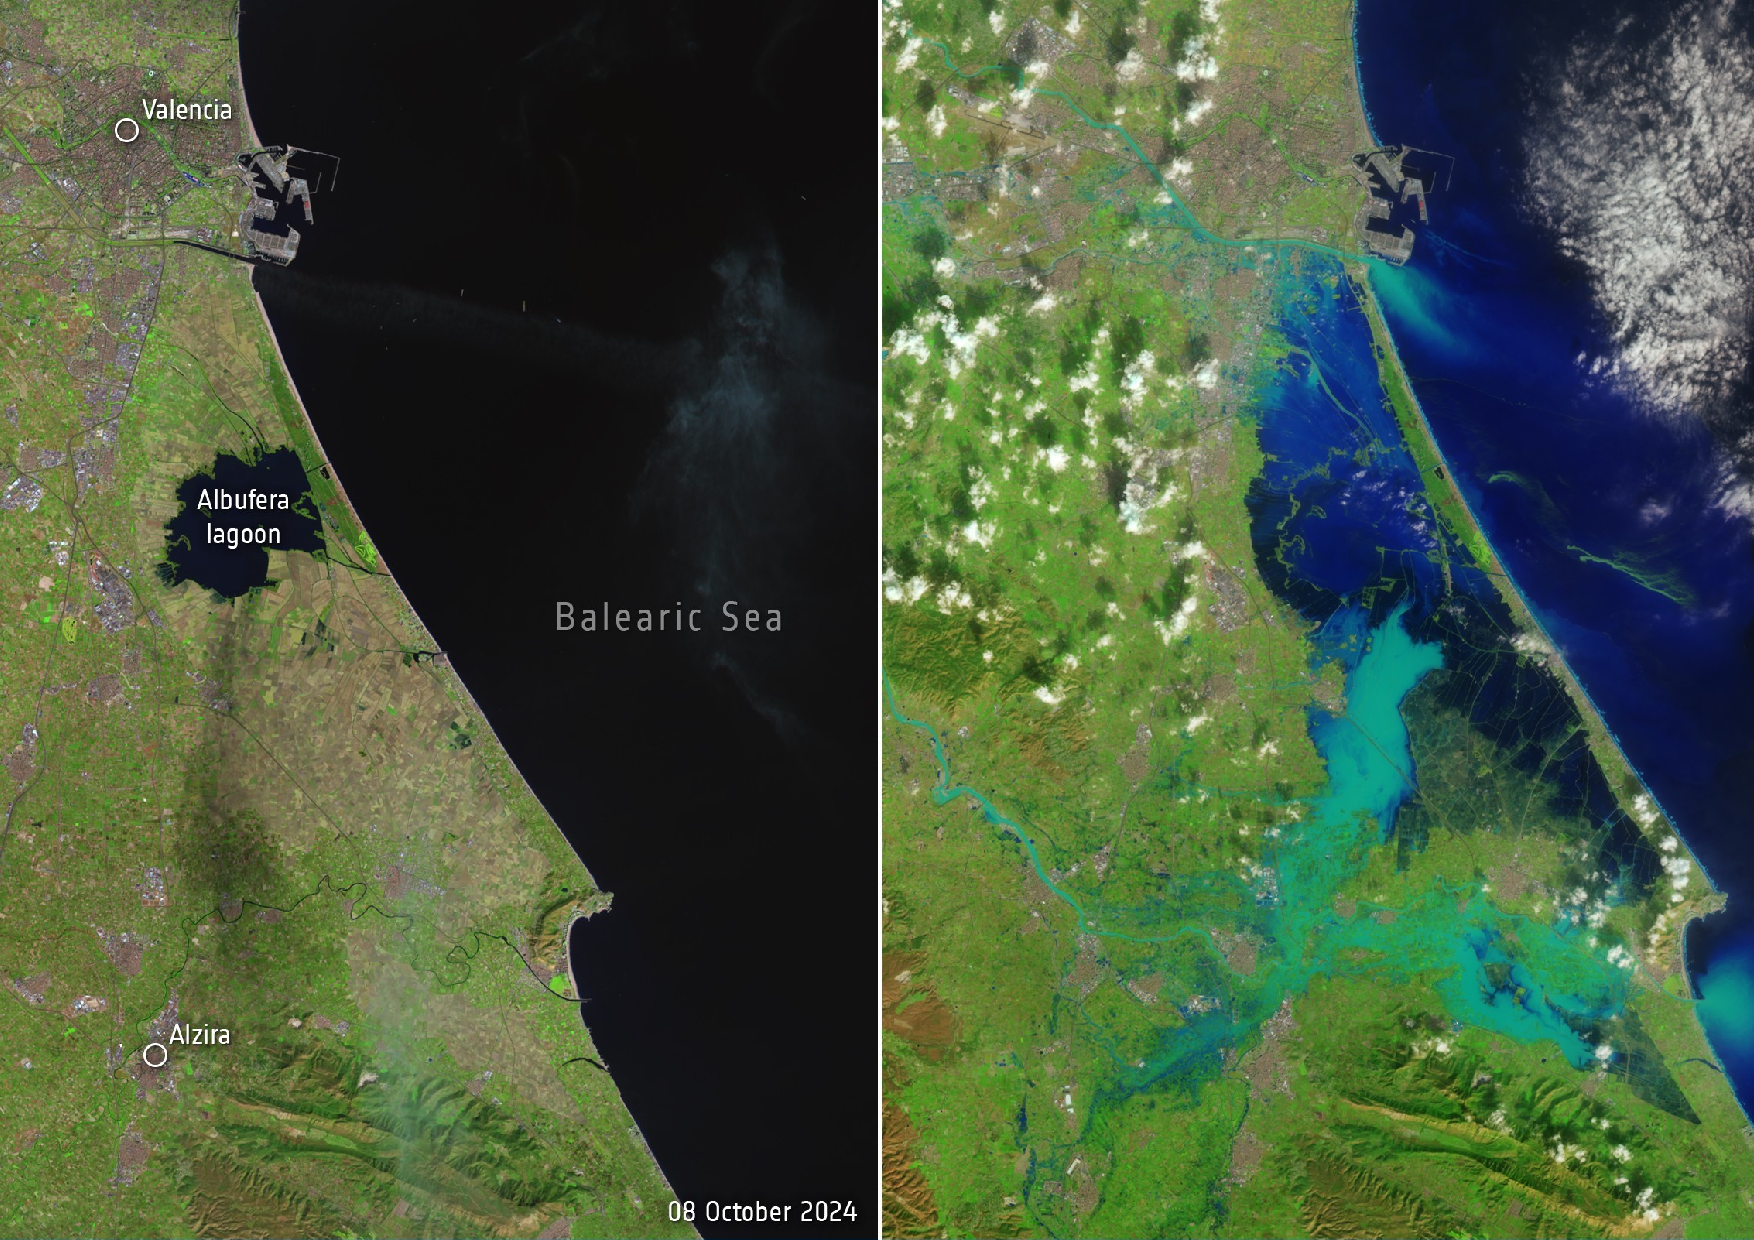
\includegraphics[width=0.7\textwidth]{C:/Users/Matteo/Shallow-Water-Equations/figs/photo_valencia.pdf}
    \caption{Before and after the floods in Valencia, Spain, October 2024.\\
            Source: \url{https://www.esa.int/ESA_Multimedia/Images/2024/10/Valencia_flood_disaster}.}\label{fig:valencia_flood}
\end{figure}
This motivates the study of the shallow water equations (SWE), a set of hyperbolic partial differential equations that describe the motion of a fluid in a shallow layer of water.
These equations are essential for understanding and simulating water dynamics in shallow water regions, such as coastal areas, rivers, and flood-prone regions.
A wide range of problems can be modeled by the SWE, such as flooding, tsunamis and dam break scenarios.
By solving the shallow water equations, we can simulate and predict the behavior of water in these regions, providing valuable insights for disaster management and emergency response.
In this work, we will derive the SWE with one spatial dimension (1D), two spatial dimensions (2D), and in spherical coordinates, which are particularly useful for modeling water flow on the Earth's surface.
We will also derive the linearized shallow water equations (LSWE) in spherical coordinates for one spatial dimension, providing a more simple framework for implementation.

The SWE can be solved using numerical methods, such as the finite volume method (FVM), which is a numerical technique for solving partial differential equations, by discretizing the domain into small control volumes and integrating the equations over these volumes.
This method is widely used in computational fluid dynamics to model fluid behavior.
In this work, we will implement the FVM in 1D and use it to solve the SWE for several scenarios, including the dam break problem.
We will extend the implementation of the FVM to 2D and solve the idealized circular dam break problem.
These FVM solvers will be validated against known test cases, as this validation is critical for future work.
We will also implement the FVM to solve the LSWE on a sphere.
For the FVM, it holds that a finer grid resolution improves solution accuracy but comes at the cost of an increased computational run time, resulting in slower simulations.
This means that while high-resolution grids can provide more accurate results, they may not be practical for real-time simulations, such as during a flood event, where fast simulations are crucial for decision-making.
This limitation motivates the investigation of data-driven approaches to solve the shallow water equations, which may offer a faster and more efficient way to simulate water dynamics while maintaining an acceptable level of accuracy.

This project investigates whether data-driven methods can provide a faster and more efficient alternative to traditional numerical methods for solving the shallow water equations.
Specifically, we will explore training a convolutional neural network (CNN) and a Fourier neural operator (FNO) to solve the SWE.
The data-driven models will be trained on the data generated from the FVM solvers, and evaluated on performance metrics such as run time, accuracy, grid transferability and their response to new initial conditions.
These initial conditions could include varying water heights, velocities, and other environmental factors that may change in real-world flood scenarios.
We will compare the advantages and limitations of the data-driven approaches against numerical methods, focusing on their potential to improve disaster responses and flood predictions.
This comparison will allow us to assess whether data-driven approaches offer a practical solution to efficiently solve the SWE.
We expect, that data-driven models may be preferred for applications requiring fast simulations, while numerical methods may be more suitable for scenarios demanding high accuracy.
An interesting aspect is to investigate how much more efficient the data-driven methods may be, compared to the traditional numerical methods, to determine to which applications they are best suited.

Additionally, we will examine the different models' abilities to make long-term predictions, meaning predicting many time steps ahead.
Numerical methods, including the FVM, solve the SWE one time step at a time, which can be computationally expensive, particularly for long-term predictions.
In constrast, data-driven models also predict one time step ahead at a time, but they may not need to be retrained for each time step.
Once trained, these models can make predictions for all time steps, potentially making them faster than numerical methods.

By analysing and comparing these approaches, this project aims to identify the contexts in which data-driven models can be a good addition or alternative to traditional numerical methods for solving the shallow water equations.


\section{Literature}
When working in this area it is inevitable to mention the work of E. F. Toro, who has written several books on the topic of Riemann solvers and the finite volume method, specifically for the shallow water equations.
In this project, we will use the books \textit{Shock-Capturing Methods for Free-Surface Shallow Flows} from 2001~\cite{Toro2001-Shock}, \textit{Riemann Solvers and Numerical Methods for Fluid Dynamics} from 2009~\cite{Toro2009-Riemann} and the rather new book from 2024 \textit{Computational Algorithms for Shallow Water Equations}~\cite{Toro2024} as references.
The books have been especially useful when deriving the shallow water equations as well as understanding and describing the finite volume method, inlcuding the Riemann solvers used in this project.
The course \textit{Advanced Numerical Methods for Environmental Models} at the University of Trento, has provided a good foundation for the numerical methods used in this project, both in terms of lecture notes and exercises~\cite{trento_course}.

Working with the SWE in spherical coordinates, the papers \textit{Well-balanced methods for the shallow water equations in spherical coordinates} by Castro et al.~\cite{Castro2017} and \textit{Physics-informed neural networks for the shallow-water equations on the sphere} by Bihlo et al.~\cite{Bihlo2022} are references for deriving the SWE in spherical coordinates.
Additionally, the lecture notes \textit{Shallow water on a sphere} by Raymond from New Mexico Tech~\cite{Raymond} and the notes from Geophysical Fluid Dynamics Laboratory~\cite{shallow_water_gfdl} have been valuable in this derivation.
Furthermore, the papers by Gavete~\cite{Gavete_2009} and Galewsky~\cite{Galewsky_2004} also provide important insights into the spherical shallow water equations.
Implementing the FVM to solve the shallow water equations in spherical coordinates is a challenging task, as exact literature on the topic is limited.
However, some sources discussing the discontinuous Galerkin scheme~\cite{Hesthaven2008} for solving the spherical shallow water equations have been useful in this context.

Convolutional neural networks (CNNs) are a well-researched area, with numerous sources available on the topic.
For this project, the paper \textit{An Introduction to Convolutional Neural Networks}~\cite{oshea2015introductionconvolutionalneuralnetworks} and the blog post \textit{A Comprehensive Guide to Convolutional Neural Networks - the ELI5 way}~\cite{chollet2017comprehensive} have been particularly helpful in explaining the theoretical foundations of the methods.
The field of Fourier neural operators (FNO) is relatively new, and as a result, there is limited literature on the topic.
However, the paper \textit{Fourier Neural Operator for Parametric Partial Differential Equations}~\cite{FNO_2021} is a key reference.
It demonstrates that FNOs are effecient and resolution independent operators for solving PDEs in scientific machine learning.
A key reason of their success is their ability to generalize to unseen data.
For more on the topic of scientific machine learning, consider the tech report~\cite{osti_1478744}.
In the last years the company Nvidia has done some very interesting work on the topic of FNOs, and they have published several blog posts on the topic.
One of the posts consider the use of spherical Fourier neural operators (SFNO) to generate weather forecasts around the globe~\cite{Nvidia2023}.
Another paper regarding SFNOs is~\cite{bonev2023-SFNO}, which generalizes FNOs on the sphere.

\newpage
\section{Thesis overview}
The rest of the thesis is structured as follows.
In \autoref{ch:theory}, we derive the shallow water equations (SWE) in 1D, 2D, and spherical coordinates.
In \autoref{ch:fvm}, we present the finite volume method (FVM) used to solve the shallow water equations, including the Riemann problem and the numerical fluxes essential for the FVM.
These chapters form the theoretical and methodological foundation for the numerical methods employed in this project, leading into the discussion of data-driven methods.

In \autoref{ch:FNO+NN}, we introduce the concepts of convolutional neural networks (CNNs) and Fourier neural operators (FNOs), explaining how these methods can be applied to solve the shallow water equations.
In \autoref{ch:method}, we describe the process of generating the data required for the data-driven methods, as we produce all the data used in this project ourselves.

Chapter~\ref{ch:numerical_results} focuses on the numerical results for the 1D and 2D SWE using the FVM.
To validate these results, we compare the FVM outputs with test cases from the literature. Validation is crucial since the data-driven models are trained on the FVM data.
We also present the numerical results of solving the 1D LSWE on a sphere using the FVM.
In \autoref{ch:data-driven-results}, we present the results for the shallow water equations using the data-driven models.
We analyze the outcomes, discuss the performance of the data-driven models, and compare them to the numerical results.

Finally, in \autoref{ch:discussion}, we discuss the findings, and in \autoref{ch:conclusion}, we conclude the thesis and propose directions for future work.


